\section{Tipos de aprendizado}

O aprendizado depende da interação entre o ambiente e aprendiz. A primeira diferença consiste no aprendizado supervisionado e não supervisionado (SHWARTZ e DAVID, 2014).

\subsection{Aprendizado supervisionado}

O aprendizado supervisionado é aquele cujos parâmetros são pré-definidos e o algoritmo procura um padrão entre os dados. As informações que serão utilizadas para treinamento já contêm informações suficientes que permitem o algoritmo inferir uma relação entre uma ou múltiplas variáveis (COLINS, 2017). A Figura 3 representa um exemplo de aprendizado supervisionado, a regressão linear.

\subsection{Aprendizado não-supervisionado}

O aprendizado não supervisionado, permite abordar problemas com pouca ou nenhuma ideia de como deverá ser o resultado (RUSSELL e NORVING, 2010). A rede tem de descobrir relações, padrões, regularidades ou categorias nos dados que lhe vão sendo apresentados e codificá-las em saídas. A Figura 4 exemplifica o aprendizado não supervisionado: a classificação de dados em dois grupos.

\subsection{Benefícios das RNA}

O poder de abstração das RNA deve-se à sua estrutura paralela e à capacidade de aprendizagem (SIMON, 2013). A estrutura paralela resulta da existência de muitos neurônios ligados em uma mesma estrutura de pesos de conexão com facilidade de adaptação a distintos tipos entrada de dados. A estrutura paralela é desejável uma vez que permite a tolerância à falha, pois se algum neurônio falhar, os efeitos na rede como um todo não serão significativos para o desempenho da rede, dado que existe outro caminho de ligação entre os nós que pode iludir a falha (HASTIE, TIBSHIRANI e FRIEDMAN, 2008).

Uma das principais características das RNA é a capacidade de aprender por meio de exemplos e de generalização, ou seja, reconhecer padrões em elementos que não foram apresentados antes, possibilitando a produção de resultado aceitável oriundo de uma nova entrada de informação (Haykin, S., 1999).

As principais propriedades que podem se destacar das redes neurais artificiais são: não linearidade, mapeamento de entrada e saída, adaptabilidade e tolerância a falhas (Haykin, S., 1999).

\subsection{Redes Neurais Artificiais}

Redes neurais artificiais foram originalmente planejadas no meio do século 20 como um modelo computacional do cérebro humano. Sua aplicação era limitada devido a limitação computacional disponível na época, além de algumas questões teóricas que não foram solucionadas por várias décadas (MURPHY, 2012).

\begin{figure}
    \caption{Neuronios}
    \centering
    \includegraphics[width=0.7\textwidth]{Textuais/Figuras/neuronios.png}
    \fonte{Autores}
    \label{fig:neuronios}
\end{figure}

É teorizado que devido a sua inspiração biológica, algoritmos baseados em redes neurais artificiais serão capazes de simular como o ser humano reconhece conceitos e objetos (COLINS, 2017).

Em uma análise matemática, as RNA podem ser explicadas como uma mapeamento não linear de um vetor de espaço de entrada para um vetor de espaço de saída, que pode ser realizado por meio de camadas de funções de ativação, em que coordenadas de entrada são somadas de acordo com o valor de seus respectivos pesos e bias  para produzir uma saída simples, ativada ou não, de acordo com o respectivo nível de acionamento (SELLI e SELEGHIM, 2007).

O conceito de rede neural artificial é basicamente introduzido pela biologia onde a rede neural tem um importante papel no ser humano. No corpo humano todo trabalho é realizado com ajuda da rede neural. Uma rede neural é uma cadeia de milhões de neurônios interconectados (SHARMA, RAI e DEV, 2012).

A terminologia rede neural é inspirada pelas operações biológicas realizadas por células especiais denominadas neurônios (Figura 5). Um neurônio é uma célula biológica especial que processa informação de um neurônio para outro com ajuda de um impulso elétrico e mudanças químicas que ocorrem no cérebro. Todo o processo de receber e enviar informação é realizado de uma forma particular: um neurônio recebe informações de outro neurônio através dos dendritos e envia informações com picos de atividade elétrica através de um longo e fino suporte conhecido como axônio que os divide em sinapses para enviá-los para outros neurônios (RUSSELL e NORVING, 2010).

%\begin{figure}
%    \caption{Célula de meuronio}
%    \centering
%    \includegraphics[width=0.7\textwidth]{Textuais/Figuras/celula.png}
%    \fonte{Autores}
%    \label{fig:celula}
%\end{figure}

As redes neurais artificiais têm o seu equivalente ao neurônio denominado nó que recebe um conjunto de entradas ponderadas, processa a sua soma com as funções de ativação $\phi$, e passa o resultado da função de ativação para o próximo nó (Figura 7) até o término da rede (Equação 18) (SHARMA, RAI e DEV, 2012).

Visualmente é equivalente a Figura 7

\subsection{Funções de ativação}

Funções de ativação são basicamente funções de transferência que são geradas pelos neurônios artificiais e envia sinal para outro neurônio artificial (SHARMA, RAI e DEV, 2012). As funções de ativação mais comuns são: Limiar, Degrau, Degrau Unitário, Linear e Logística (Figura 8). 

Existem diversas funções de ativação, como por exemplo a função linear (Equação  19), também denominada função identidade.

Outra função de ativação é a função sigmoid (Logística) representada pela Equação 19.

Uma função muito utilizada é a tanh, representada pela Equação 20.

A possível criação de uma rede neural ocorre por meio do encadeamento dos nós. Usualmente esse processo é realizado utilizando camadas, as saídas de um nó estão conectadas a entrada dos nós da próxima camada (ABADI, 2015).

O objetivo de aproximações de funções é treinar uma rede neural que seja capaz, a partir de um conjunto de dados entrada-saída, de mapear uma determinada relação funcional que contemple o universo de amostras sob análise. O treinamento, nesse caso, envolve o aprendizado dos pesos de borda corretos para produzir a saída de destino, dada uma entrada (SHWARTZ e DAVID, 2014). A rede e seus pesos treinados formam uma função (denominada h) que operam sob dados de entrada. Com a rede treinada, é possível produzir previsões para valores de entrada previamente desconhecidos.

É possível treinar uma rede neural para realizar regressão ou classificação. Nesse trabalho iremos abordar somente a regressão linear. 

\begin{figure}
    \caption{Representação de uma regressão e classificação}
    \centering
    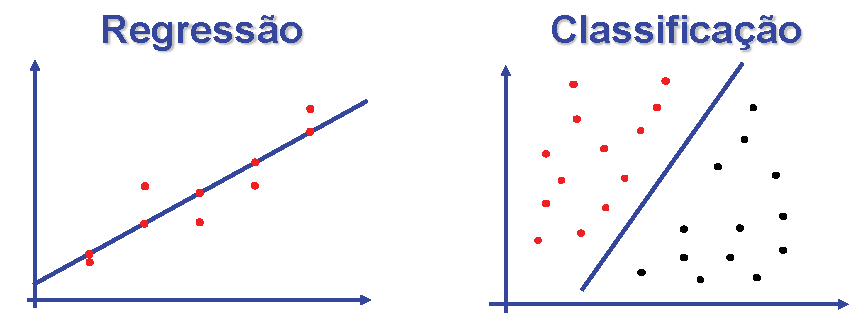
\includegraphics[width=0.8\textwidth]{Textuais/Figuras/ai.pdf}
    \fonte{Autores}
    \label{fig:reg-class}
\end{figure}

Regressão linear é a forma mais simples de regressão (RUSSELL e NORVING, 2010). Modelamos o nosso sistema como combinações lineares de features para produzir uma saída.

A RNA torna-se responsável por encontrar os pesos que geram o melhor resultado para os dados de treinamento. Um modo de verificar a qualidade da aproximação é utilizando o método dos mínimos quadrados (também conhecido como Loss) (HOPE e LIEDER, 2017).

Para poder realizar o melhor ajuste é preciso minimizar o valor de L(w). Esse método possui uma solução analítica, mas em geral pode-se resolver utilizando o método do gradiente descendente (RUSSELL e NORVING, 2010).

A rede neural mais simples utiliza o método dos mínimos quadrados para realizar uma regressão linear como mostra a Figura 10. 

Essa rede recebe como entrada de dados duas features xi(1) e xi(2), os pesos das features como w1 e w2 e os soma, e como saída tem-se a previsão yi. Pode-se considerar uma rede neural com n parâmetros de entrada, porém a rede deve conter n pesos, sendo equivalente um peso para cada entrada. Para poder determinar a qualidade de aproximação é possível utilizar o método dos mínimos quadrados (MOHRI, ROSTAMIZADEH e TALWALKAR, 2012).

Abadi (2015) utiliza o método do gradiente descente para minimizar os erros em relação aos dados de treinamento. Primeiramente deriva-se o gradiente descendente em relação a um determinado peso wj->k

Nesse ponto, calcula-se o gradiente da função da rede em relação ao peso da derivada parcial. 

O gradiente em relação a w1 é apenas x1, e o gradiente em relação a w2 é apenas x2, dessa forma o gradiente é dado pela Equação 28.

Agora é possível atualizar os pesos utilizando o gradiente descendente padrão

Onde ``eta`` é o passo.

\subsection{Testando a RNA}

Com a rede treinada, testar consiste em obter a previsão para cada ponto xi utilizando a função h(xi, w). O erro pode ser calculado da mesma forma do treinamento utilizando a Equação 30.

\subsection{Teorema Universal da Aproximação}

O Teorema Universal da Aproximação garante que uma Rede Neural Artificial do tipo Função Radial de Base pode ser treinada para ajustar, satisfatoriamente, qualquer função contínua definida em um conjunto fechado (HAYKIN, 1999).